\documentclass[11pt]{article}
\usepackage[spanish]{babel}


%%%%%%%%%%%%%%%%%%%%%%%%%%%%%%%%%%
%%%%%%%%%%%%%%%%%%%%%%%%%%%%%   %%
%%        Datos Trabajo     %%  %%
%%%%%%%%%%%%%%%%%%%%%%%%%%%%%%%%%%
\newcommand{\titulo}[0]{Reto 4. FINTECH}
\newcommand{\materia}[0]{Finanzas Personales v1}


%%%%%%%%%%%%%%%%%%%%%%%%%%%%%%%%%%
%%%%%%%%%%%%%%%%%%%%%%%%%%%%%%%%%%
\usepackage{amssymb}
\usepackage{enumerate}
\usepackage{geometry}
\usepackage{mathtools}
\usepackage{multicol}
\usepackage{soul}

\usepackage{graphicx}
	\graphicspath{ {assets/} }

\usepackage{hyperref}
	\hypersetup{
			pdftex,
		        pdfauthor={bench},
		        pdftitle={...},
		        pdfsubject={...},
		        pdfkeywords={UVEG},
		        pdfproducer={Latex with hyperref, Ubuntu},
		        pdfcreator={pdflatex, or other tool},
			colorlinks=true,
				linkcolor=[rgb]{0,0,0.45},
				urlcolor=cyan,
				filecolor=green,
				citecolor=blue}

%%%%%%%%%%%%%%%%%%%%%%%%%%%%%%%%%%
%%%%%%%%%%%%%%%%%%%%%%%%%%%%%%%%%%

\title{\titulo}

\author{ Universidad Virtual del Estado de Guanajuato \textbf{UVEG} \\ 
\materia \\ Benjamín Rivera \\ 19015478 }
\date{\textit{Fecha de entrega:} \today}


%%%%%%%%%%%%%%%%%%%%%%%%%%%%%
%%        Documento         %%
%%%%%%%%%%%%%%%%%%%%%%%%%%%%%%%
\begin{document}
	\maketitle
	
	\par Yo decidí descargar y probar la aplicación \textit{Mobills Finanzas y Presupuesto - Control de Gastos}, la cual se encuentra disponible en la tienda oficial de aplicaciones de Android (la Play Store); un detalle con esta aplicación es que no se si se encuentre disponible para las demás plataformas de dispositivos mobiles, por lo que no se que tan accesible sea desde ese aspecto. Esta aplicación pertenece y fue desarrollada por \textit{Mobills Inc.} que es una compañía que se encarga de desarrollar diversas aplicaciones, productos y soluciones de carácter financiero, la mayoría de ellas con buenas referencias en la tienda de aplicaciones y que parecen tener buena calidad. 
	
	\par Esta aplicación que yo estuve probando, durante aproximadamente una semana, y utilizando por una semana tiene dos versiones, la completamente gratuita y la de pago o premium (cuyo costo, de aproximadamente 500 pesos al mes, me parece bastante accesible). Las diferencias entre estas dos son mínimas y cubren principalmente una ampliación en la capacidad de la cantidad de datos de las mismas funcionalidades que aporta la básica.
	
	\par Respecto a lo que se refiere a la parte práctica y estética, la aplicación me parecio bastante intuitiva, accesible y práctica además de que visualmente la describiría como bonita y minimalista. Respecto a la versión que probé, que fue la gratuita, sus funciones me parecieron más que suficiente para mi, actualmente limitada, actividad financiera (y claro durante mi periodo de prueba). Aunque considero que para un uso más intensivo si se requerirían algunas de las funciones de la versión de paga que, como ya mencione anteriormente, e parece accesible y que sería un gasto que valdría la pena para poder cuidar constantemente nuestra salud financiera. En la aplicación se pueden registrar los gastos e ingresos, clasificar estos dos para mantener un orden de los mismos, además de conectar algunas cuenta bancarias (por que no todos los bancos prestan las mismas facilidades, aunque por suerte ya la mayoría se están actualizando para permitir esta clases de aplicaciones) para facilitar el mantenimiento y la integridad de los registros de los ingresos y los egreso que se efectúan con estas. 
	
	\par Dentro de sus funcionalidades también estan la creación de presupuestos, que se necesitaba para completar de manera exitosa eta actividad. Tengo algunas quejas respecto a esta funcionalidad, ya que no era del todo clara (o al menos no para mi) respecto al método de creación de los mismos y de las cantidades y plazos que te permitía ir creando a lo largo del proceso.
	
	\begin{figure}[htp]
		\centering
		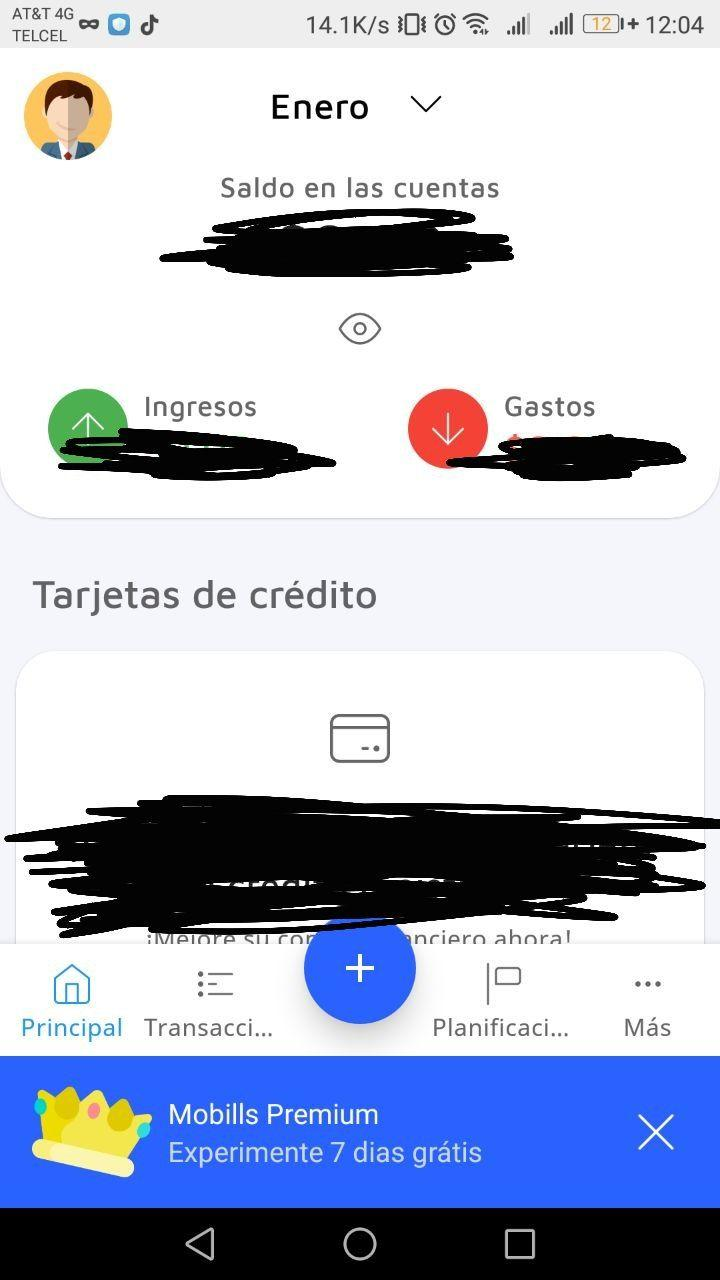
\includegraphics[width=0.3\textwidth]{assets/R4_U2-1.jpg}
		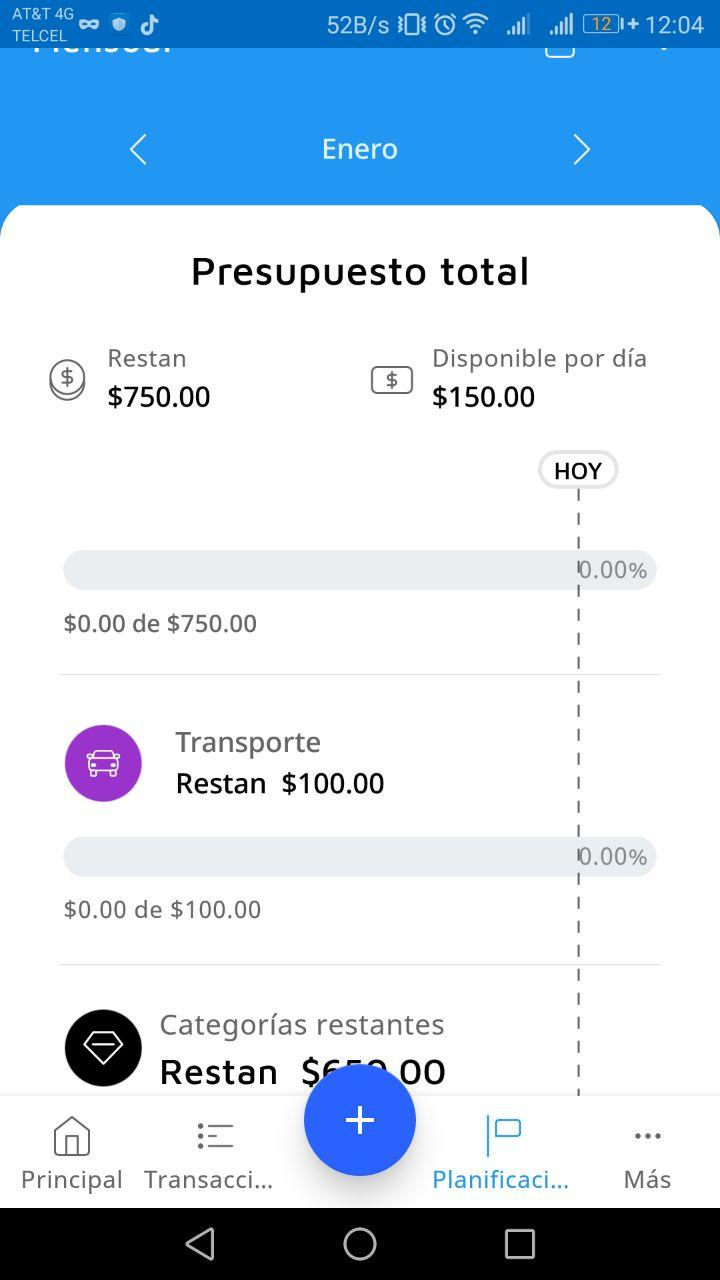
\includegraphics[width=0.3\textwidth]{assets/R4_U2-3.jpg}
		\caption{Capturas de pantalla de la aplicación.}
		\label{Capturas}
	\end{figure}
	
	\begin{figure}[htp]
		\centering
		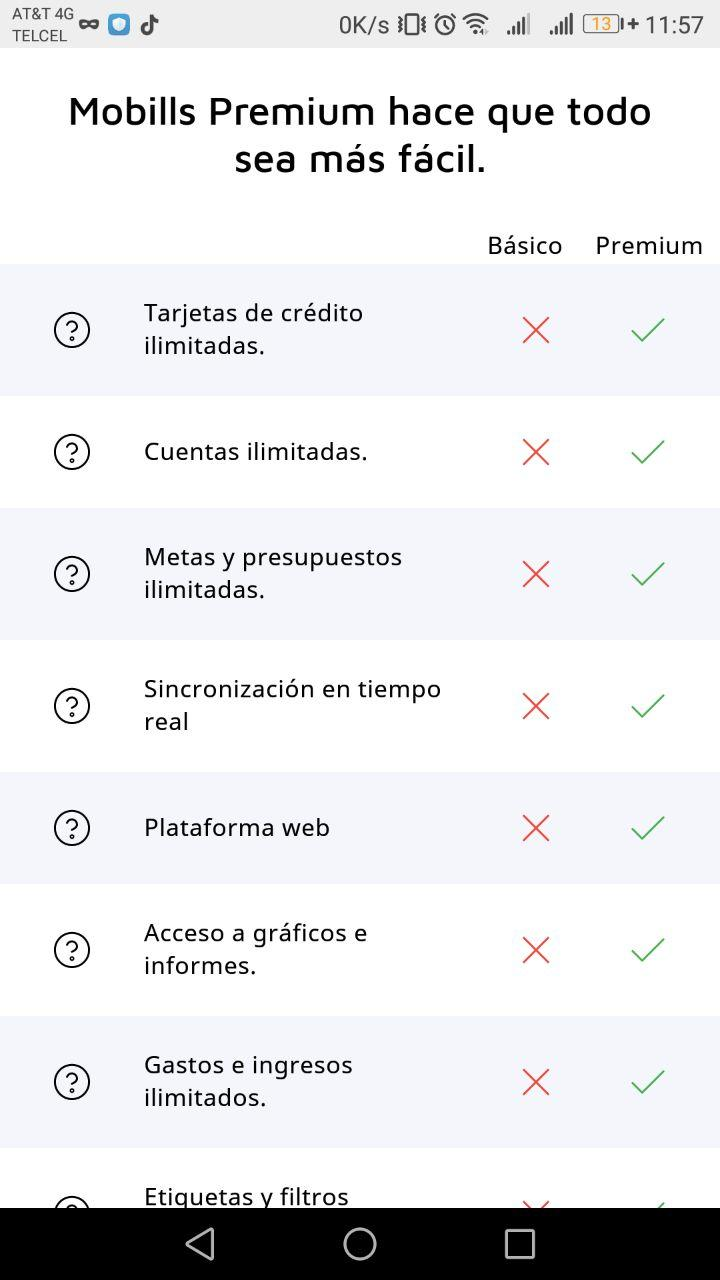
\includegraphics[width=0.4\textwidth]{assets/R4_U2-2.jpg}
		\caption{Algunas diferencias entre versión gratuita y \textit{premium}.}
		\label{Capturas}
	\end{figure}
	
	d)Redacta con tus palabras un párrafo de conclusiones de al menos 300 palabras. Comparte tu opinión sobre la utilidad de las herramientas abordadas, y cómo esta actividad te apoya en tus planes financieros personales.

	\par En general creo que la aplicación es práctica e ideal para mantener un registro de los gastos e ingresos que llevamos en el tiempo. También para el desarrollo y concientización de presupuestos y metas; ya que, después de jugar un rato y entender la aplicación, la definición de estos dos tipos de objetivos es específica, además de que los recordatorios de la misma son constantes y no demasiado intrusivos (en el punto ideal para mi gusto). Para el uso del día a día yo recomendaría ampliamente la contratación de la versión premium; tanto para el apoyo de los desarrolladores, como porque la ampliación de las funcionalidades lo vale.
	
	\par Respecto al ejercicio, después de haberlo llevado a acabo por una semana, me doy cuenta de que llevar un registro, tanto de los ingresos como de los gastos, y crear presupuestos para las metas es una actividad que consume poco tiempo y que en la misma actividad nos ayuda para apoyar constantemente a nuestra salud financiera. Por sobre esto, el uso de las tecnologías de la información (TIC's), es algo que facilita aún más el desarrollo de actividades de este estilo; y con el constante contacto con estas, las notificaciones que nos úede mandar y con un poco de disciplina de nuestra parte, el logro de metas y logros que dependen de situaciones financieras (como la compra de un auto o el aseguramiento de la educación de mis hijos) es perfectamente alcanzable (siempre y cuando no haya demasiada suerte en nuestra contra).
	
	\par En conclusión podemos decir que; el uso de las herramientas \textit{ya}	disponibles, en los dispositivos relacionados con las \textit{TIC's}, y el desarrollo de actividades como el control de gastos, la presupuestación de objetivos y la disciplina de nuestro bolsillo; son actividades accesibles para la mayoría de nosotros y que apoyan de manera positiva al mantenimiento de una buena salud financiera. Y el mantener una buena salud financiera es algo que apoya positivamente tanto a nosotros, como a aquellos más cercanos a nosotros y, principalmente, a aquellos que dependen de nosotros económicamente.


%%%%%%%%%%%%%%%%%%%%%%%%%%%%%%%%
%%         Bibliografia        %%
%%%%%%%%%%%%%%%%%%%%%%%%%%%%%%%%%%
\newpage
	\begin{thebibliography}{X}
	
		\bibitem{1} 9 aplicaciones para mantener bajo control los gastos | Forbes España. (s/f). Recuperado el 27 de enero de 2021, de \url{https://forbes.es/empresas/33645/9-aplicaciones-mantener-control-los-gastos/}
		\bibitem{2} Alonso, C. J. (2017, octubre 25). 9 aplicaciones para mantener bajo control los gastos. Forbes España. \url{https://forbes.es/empresas/33645/9-aplicaciones-mantener-control-los-gastos/}
		\bibitem{3} Finerio | App de finanzas personales y control de gastos. (s/f). Recuperado el 27 de enero de 2021, de \url{https://finerio.mx/}
		\bibitem{4} Fintonic. (s/f). Organiza tu Dinero y Ahorra con la App de Fintonic. Fintonic. Recuperado el 27 de enero de 2021, de \url{https://www.fintonic.com}
		\bibitem{5} Fintonic, Revolut, Goin...7 apps gratuitas que te ayudarán a ahorrar dinero. (s/f). Recuperado el 27 de enero de 2021, de \url{https://www.20minutos.es/noticia/4075952/0/7-apps-gratuitas-para-controlar-tus-finanzas-que-te-ayudaran-a-ahorrar/}
		
	\end{thebibliography}

\end{document}